\documentclass{article}
\usepackage[utf8]{inputenc}
\usepackage{graphicx}
\usepackage{mathtools}
\usepackage{amssymb}
\usepackage{amsmath}
\usepackage{macros}
\usepackage{color}

\begin{document}

\section{Egenskaper hos deriverbara funktioner}
Vad talar derivatan om för oss om funktionens egenskaper? Derivatans tecken visar
funktionens lutningskoefficient. Om derivatan är positiv i varje punkt så är funktionen
strikt växande.

\subsection{Exempel}
"För vilka $x$ är $f(x)=x^2$ strängt växande?"
%\img{img/x.png}
$$f(x)=x^2$$
$$f'(x)=2x$$
$x>0$?
$x<=0$?
Räknas $x=0$ med?

\subsection{Notera definitionen (strängt växande)}
$f$ är strängt växande på ett intervall I om $f(x)<f(y)$ gäller då $x,y\in I$ och $x<y$.\\

Observera:
\begin{itemize}
  \item Definitionen av växande nämner inte begeppet derivata.
  \item Det handlar bara om jämförelse mellan funktionsvärden i olika punkter.
  \item "Strängt växande i en enstaka punkt" är inte ett meningsfullt begrepp!
\end{itemize}

% forts av ex
Frågan ovan är alltså dåligt formulerad!
En bättre fråga: "Vilket är det största intervallet där $f(x)=x^2$ är strängt växande?"\\
Svar: $[0,\infty[$ ($x\le 0$, alltså)

\subsection{Definition (lokalt minimum)}
Funktionen $f$ har lokalt minimum (respektive strängt lokalt minimum) i punkten $a\in D_f$ om det
finns ett öppet intervall $I$ kring a sådant att $f(a)\le f(x)$ (respektive $f(a)<f(x)$) när
$a\neq x \in I \cap D_f$.\\
(För (strängt) lokalt maximum, vänd på olikheterna.)\\

\subsubsection{Terminologi}
Lokalt maximi- och minimipunkter kallas kollektivt för lokala extrempunkter.

\subsection{Exempel}
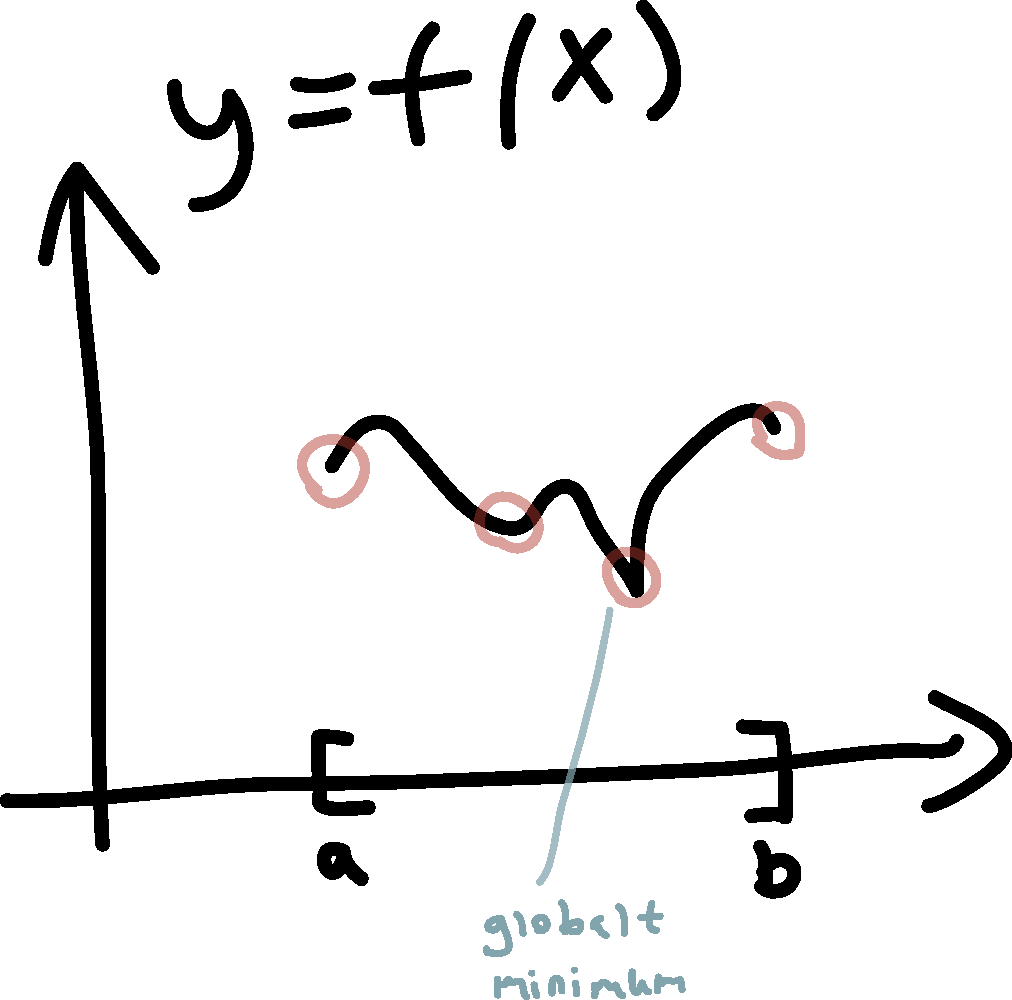
\includegraphics[scale=0.4]{img/graph1.pdf}\\
$f$ har 4st lokala minima.

\subsection{Sats}
Om $a$ är en lokal extrempunkt för $f$, och $f'(a)$ existerar, så är $f'(a)=0$.

\subsection{Bevis}
Om a är en lokal minimipunkt så är $f(a+h)-f(a)\ge 0$ för h nära 0.
Om $f'(a)$ existerar så är alltså
$$
\begin{cases}
f'(a) = f'_+(a)=\lm h {0^+} \f{f(a+h)-f(a)}h \ge 0\\
f'(a) = f'_-(a)=\lm h {0^-} \f{f(a+h)-f(a)}h \le 0
\end{cases}
\im f'(a) = 0
$$
(lokalmaximi på samma sätt)
\qed

\subsection{Definition}
En punkt där $f'(a) = 0$ kallas för en stationär punkt för $f$.

\subsection{Exempel}
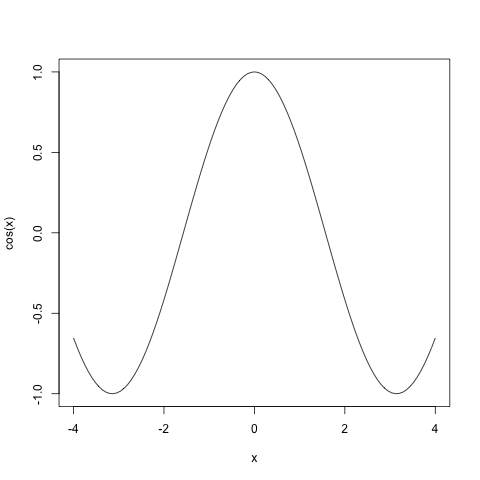
\includegraphics[height=60mm, width=60mm]{img/cos.png}\\
$f(x) = \cos x$ har (globalt) minimum i $x=\pi$ och är även deriverbar där. Enligt satsen (1.5) ovan måste
därmed $f'(\pi)$ vara noll, och så är det ju: $f'(x)=-\sin x \im f'(\pi) = 0$.

\subsection{Exempel}
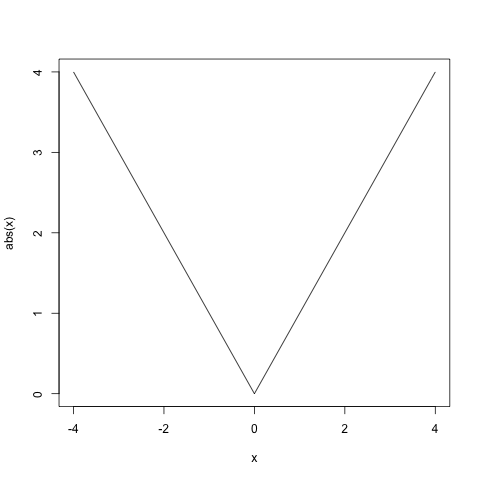
\includegraphics[height=60mm, width=60mm]{img/abs.png}\\
$f(x)=\abs x$ har minimum i $x=0$, men $x=0$ är inte en stationär punkt eftersom $f$ inte är deriverbar där.

\subsection{Exempel}
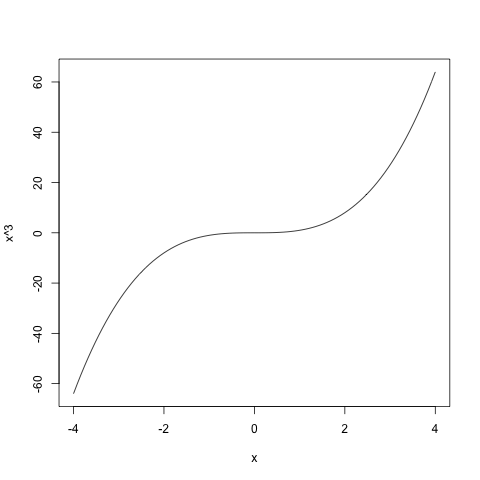
\includegraphics[height=60mm, width=60mm]{img/x3.png}\\
$x=0$ är en stationär punkt för $f(x)=x^3$ ($f'(x)=3x^2\im f(0)=0$),
men det är inte en lokal extrempunkt (utanen terrasspunkt).

\section{Medelvärdessatsen och dess konsekvenser}
\subsection{Sats}
Antag att $f$ är kontinuerlig på $[a,b]$ och deriverbar på $]a,b[$.\\

\subsubsection{(a) Rolles sats}
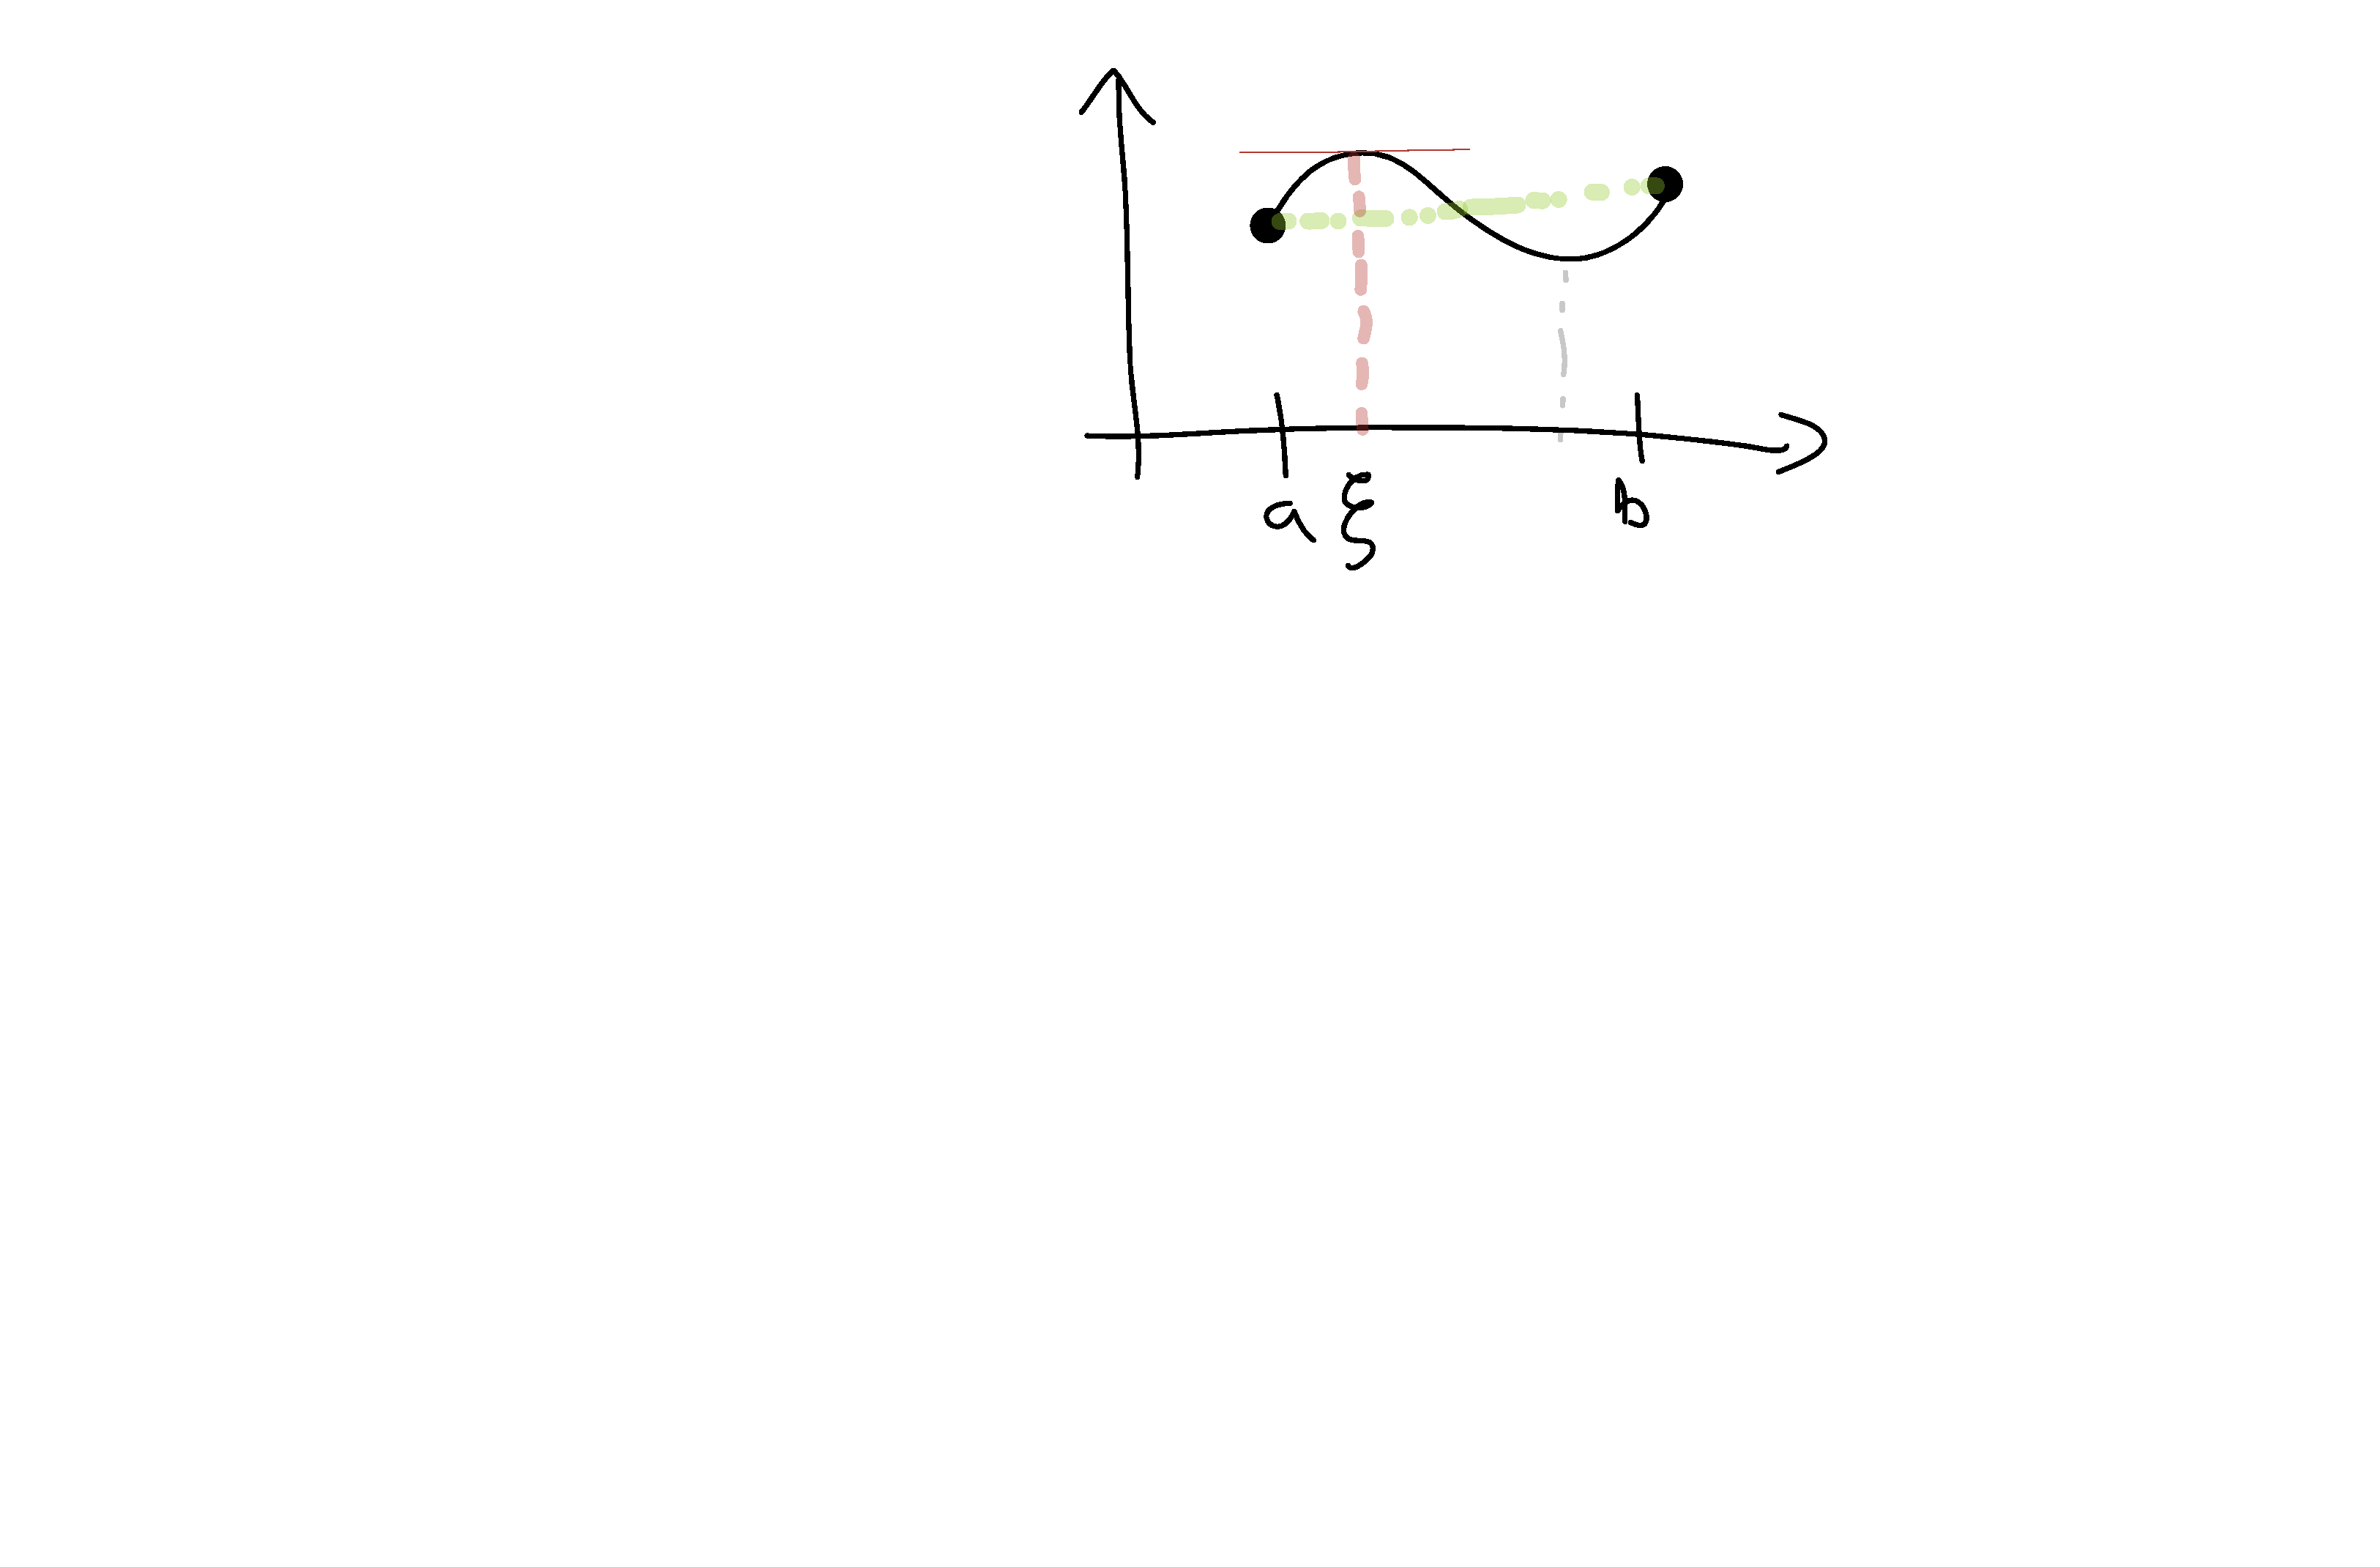
\includegraphics[scale=0.2]{img/graph2.pdf}\\
Om $f(a)=f(b)$ så finns (minst) en punkt $\xi\in ]a,b[$ där $f'(\xi) = 0$

\subsubsection{(b) Medelvärdessatsen för derivator}
Det finns (minst) en punkt $\xi\in ]a,b[$ där $f(\xi)=\f{f(b)-f(a)}{b-a}$
(dvs $\dxf (\xi) = \f{\Delta f}{\Delta x}$)
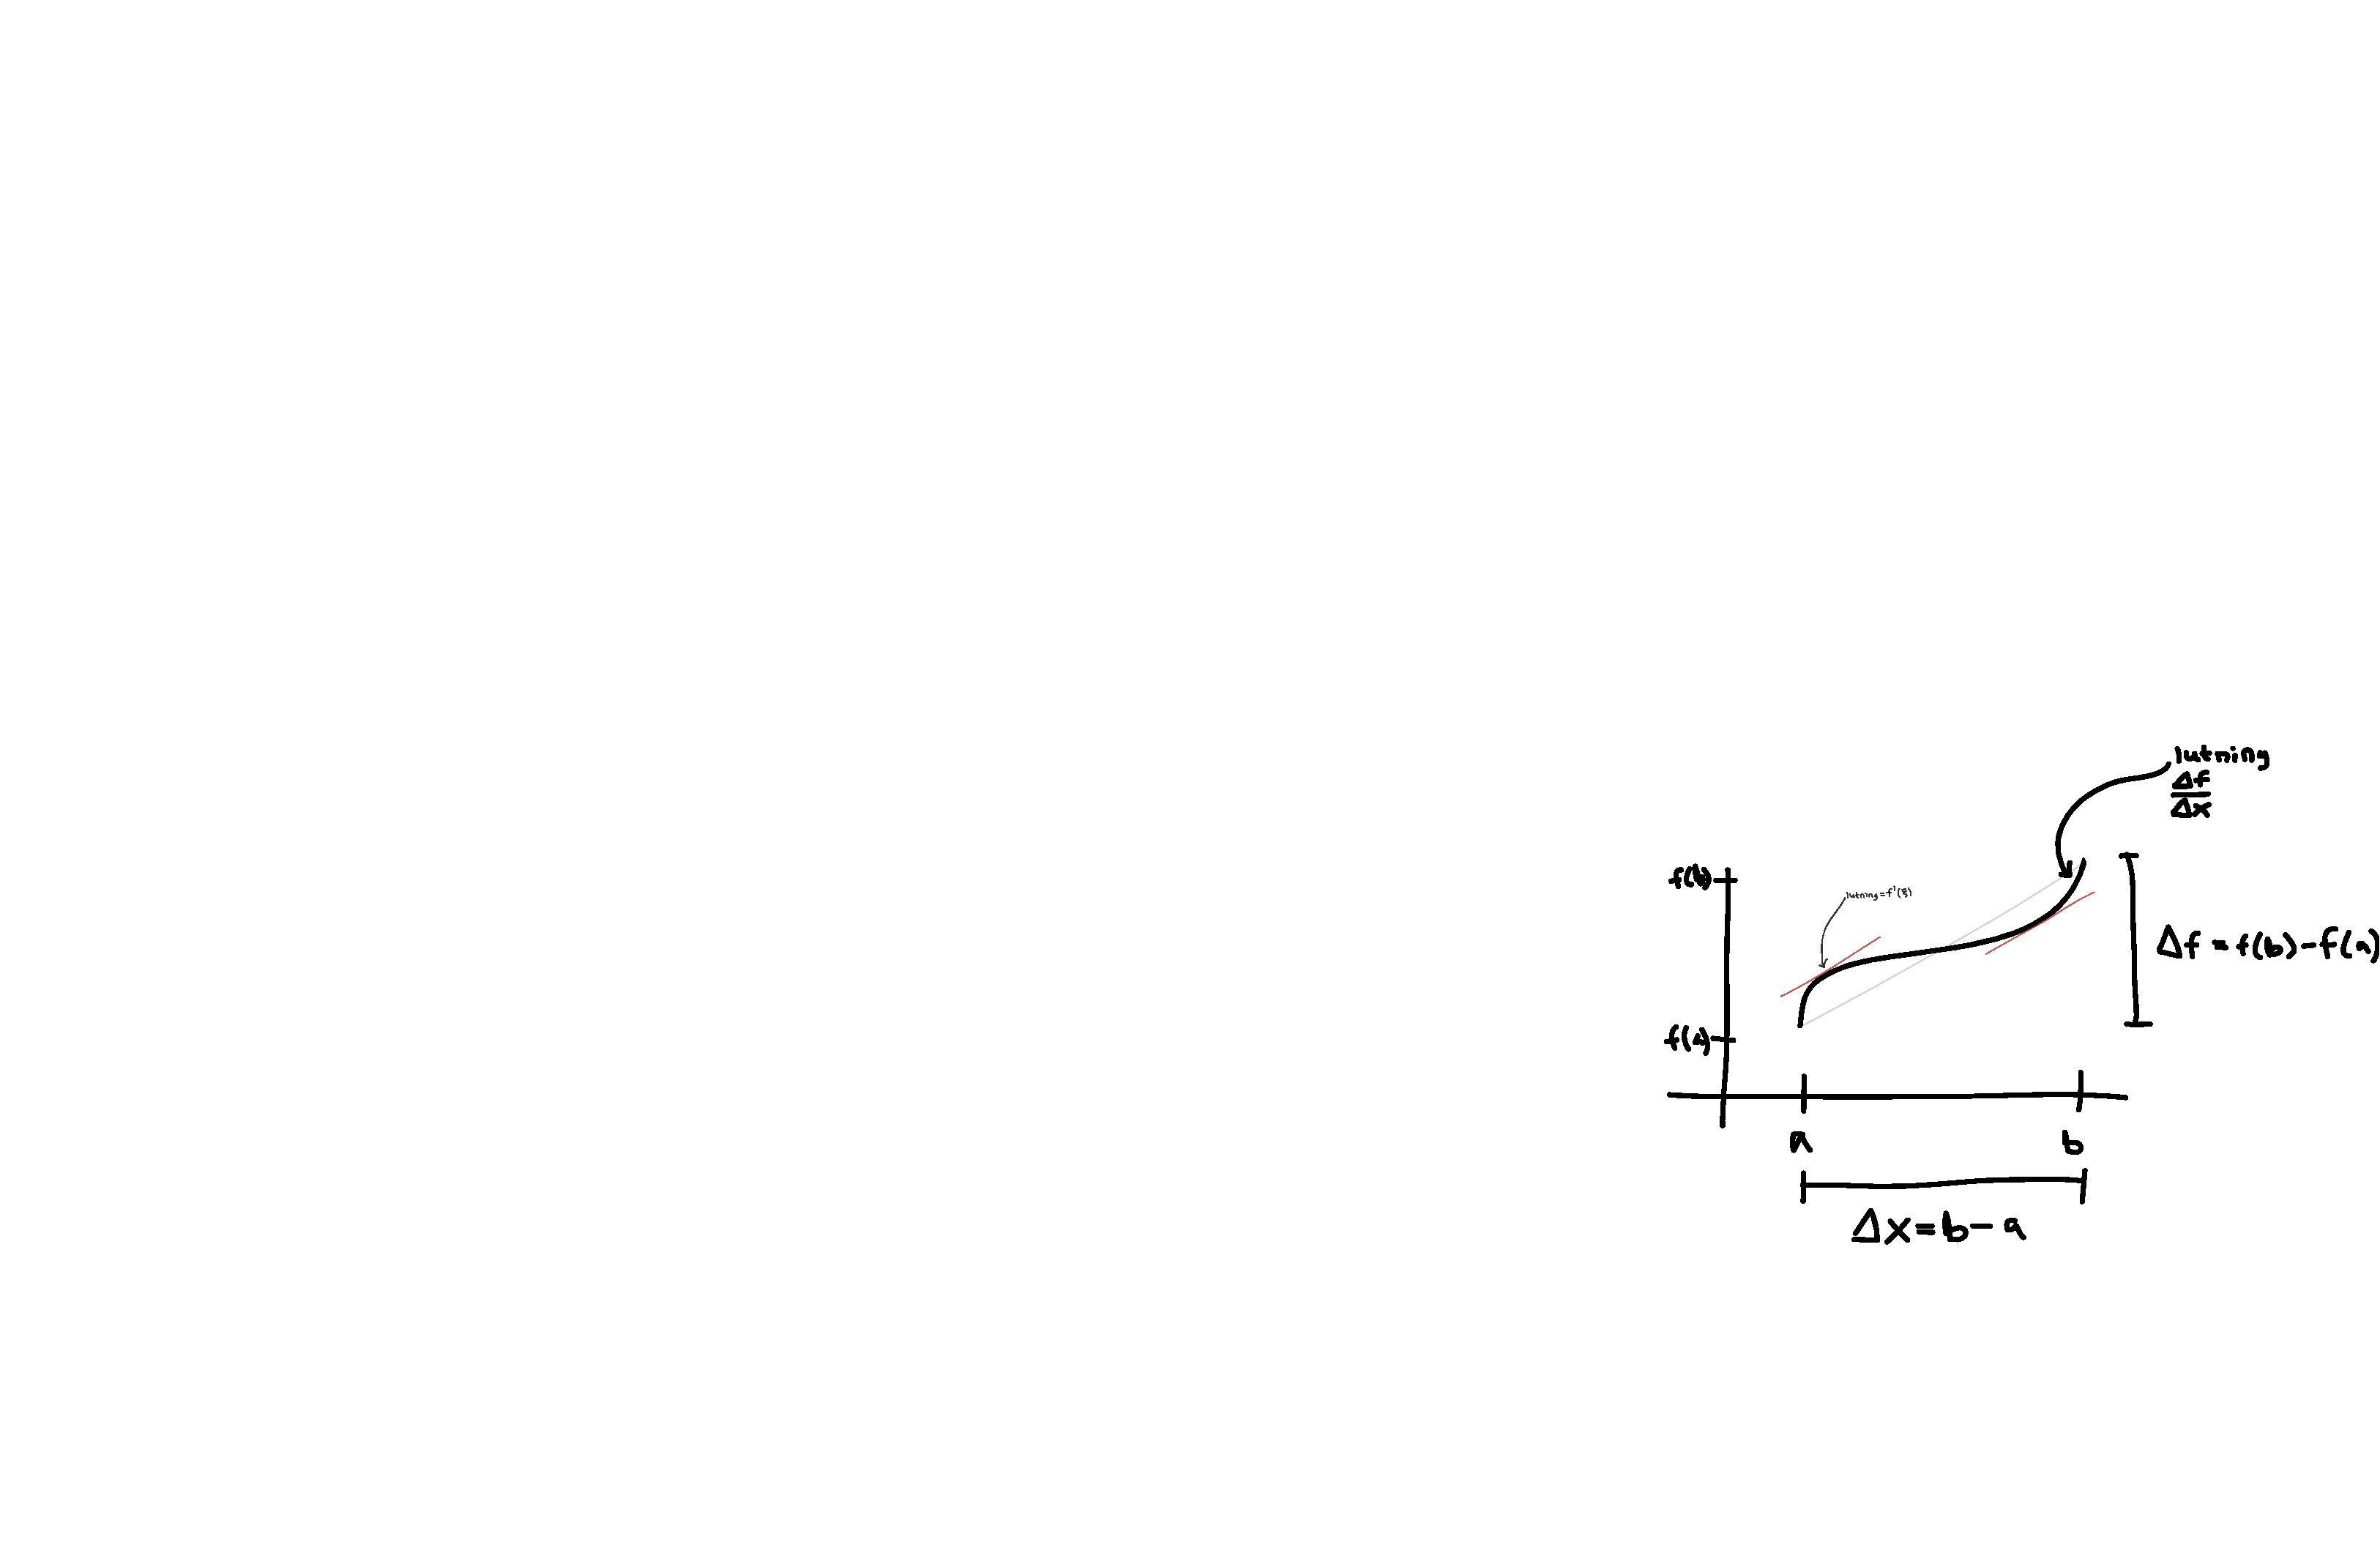
\includegraphics[scale=0.5]{img/graph3.pdf}\\

\subsubsection{(c) Derivatatestet}
Om $f' > 0$, för alla $x$, (respektive $f'=0$ respektive $f'<0$) på $]a,b[$ så är $f$ strängt växande
(respektive konstant respektive strängt avtagande) på $[a,b]$\\

(Om $f' \ge 0$, för alla $x$, (respektive $f'\le 0$) så är $f$ växande (respektive avtagande), men inte
nödvändigtvis strängt)

\subsubsection{Anmärkning}
Observera att en strängt växande funktion inte måste ha en positiv derivata överallt!
Derivatan kan vara noll i enstaka punkter. (Kom ihåg exemplet $f(x)=x^3$.)

\subsection{Bevis}
\subsubsection{(a)}
Intervallet $[a,b]$ är kompakt (dvs slutet och begränsat), och $f$ är kontinuerligt på $[a,b]$
enligt föruts., så $f$ har ett största och ett minsta värde. Såvida
inte $f$ är konstant på $[a,b]$ så måste minst en av de extrempunkterna ligga i det inre av intervallet,
alltså i $]a,b[$, där $f$ enligt föruts. är deriverbar, och enligt tidigare sats så
är $f'(\xi)=0$ i en sådan punkt $\xi$. (Och om $f$ är konstant på $[a,b]$ så är $f'(\xi)=0$ för alla
$\xi\in ]a,b[$)

\subsubsection{(b) (skiss, se boken)}
Sätt $g(x) = f(x)-\f{\Delta f}{\Delta x} \times (x-a)$. Då är
$$g(a)=\cdots=g(b)$$
och
$$g'(x)=f'(x)-\f{\Delta f}{\Delta x} \times 1$$
Del (a) ger oss $\xi$ så att $g'(\xi)=0$, dvs $f'(\xi)=\f{\Delta f}{\Delta x}$

\subsubsection{(c)}
Ta två godtyckliga punkter $x_1<x_2$ i $[a,b]$ och tillämpa del (b) på intervallet $[x_1, x_2]$:
$$ f'(\xi) = \f{f(x_2)-f(x_1)}{x_2-x_1} $$
för något $\xi \in ]x_1,x_2[$\\

dvs $f(x_2) - f(x_1) = f'(\xi) \times (x_2-x_1)$ för något $\xi \in ]x_1, x_2[$.\\\\
Om nu $f'>0$ överallt så vet vi att $f'(\xi)>0$ så att $f(x_2)-f(x_1)>0$, dvs $f$ är strängt växande.\\
Om nu $f'=0$ överallt så vet vi att $f'(\xi)=0$ så att $f(x_2)-f(x_1)=0$, dvs $f$ är konstant.\\
Om nu $f'<0$ överallt så vet vi att $f'(\xi)<0$ så att $f(x_2)-f(x_1)<0$, dvs $f$ är strängt avtagande.

\subsection{Exempel}
Rita grafen för $f(x)=x^2\times e^{-x}, (x\in\R)$.\\
Gränsvärden:
$$ f(x)\to 0, x\to\infty, \left(\f{x^2}{e^x}\to 0\right)$$
$$ f(x)\to\infty, x\to -\infty $$
Obs även att $f(x)\ge 0$ för alla x, och att $f(x)\approx x^2\times 1$ då $x\approx 0$.
$$ f'(x) = 2xe^{-x} + x^2(-e^{-x}) = (2x-x^2)e^{-x} = x(2-x)e^{-x} $$

\begin{tabular}{ l l p{7mm} l p{7mm} l }
  && 0 && 2 &\\ \hline
  $x$ & - & 0 & + & + & + \\
  $2-x$ & + & + & + & 0 & - \\
  $e^{-x}$ & + & + & + & + & + \\ \hline
  $f'(x)$ & - & 0 & + & 0 & - \\
  $f(x)$ & $\searrow$ & lok. min. & $\nwarrow$ & lok. max. & $\searrow$
\end{tabular}

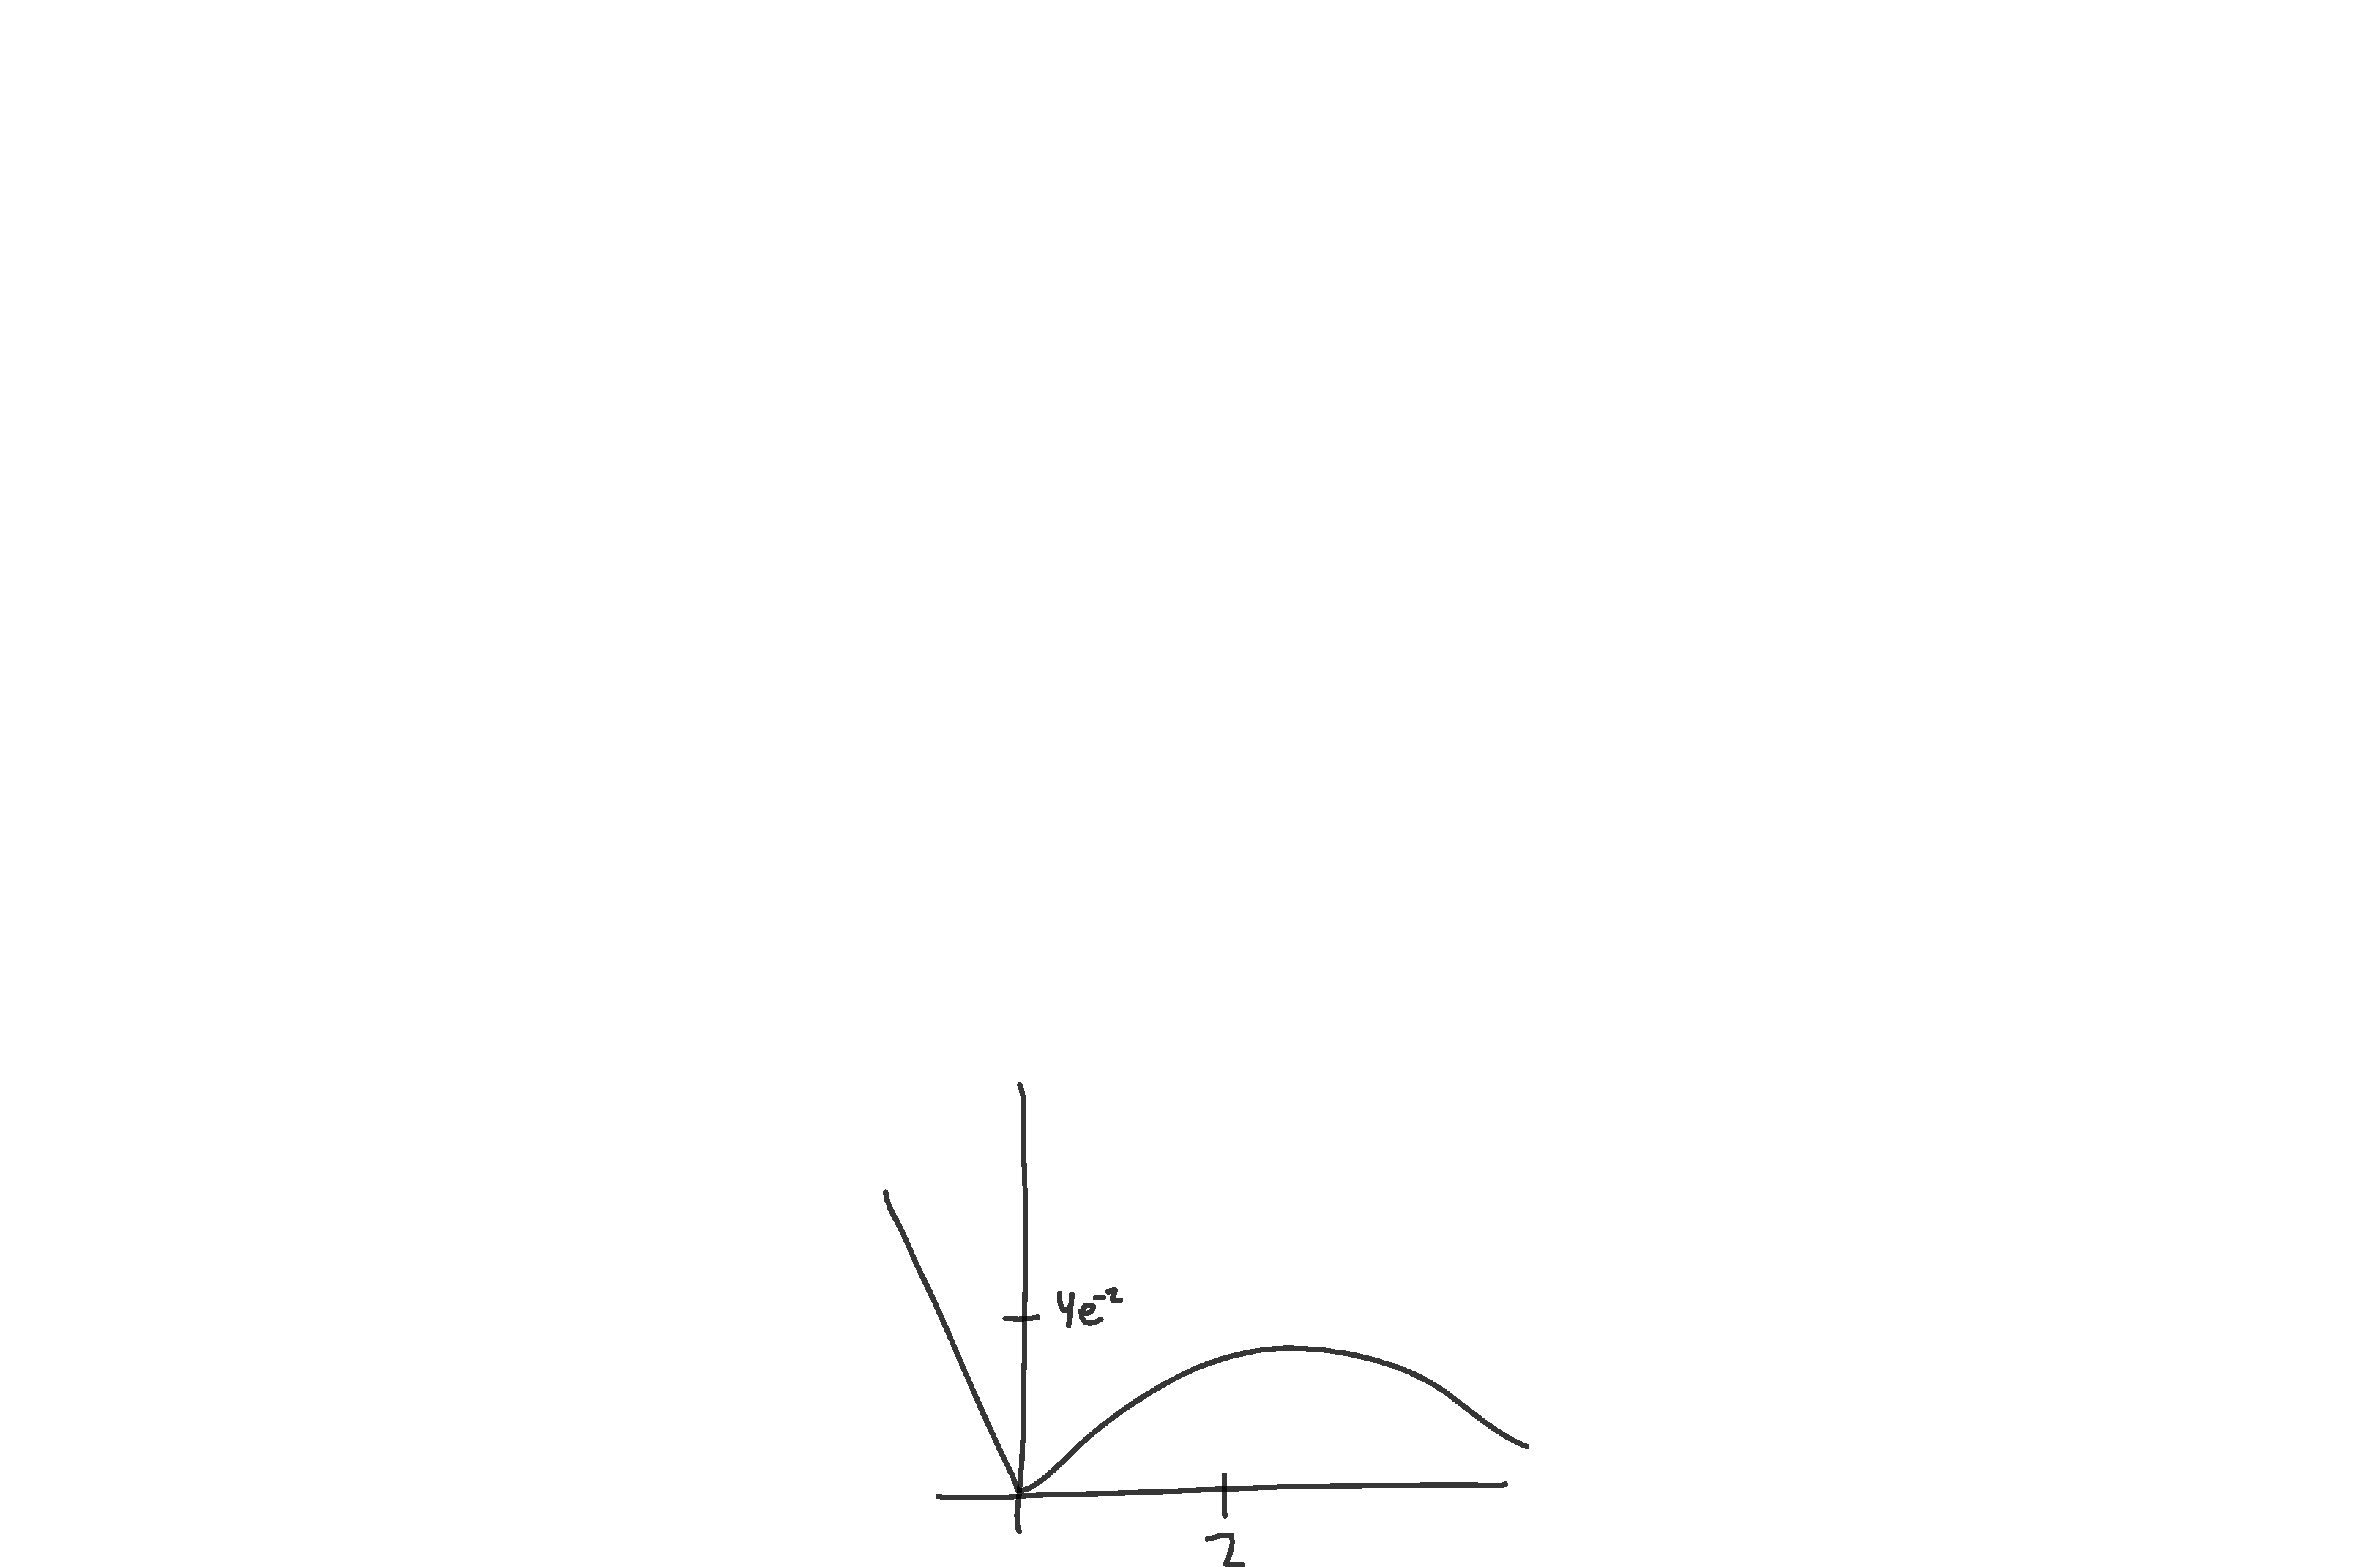
\includegraphics[width=\textwidth]{img/graph4.pdf}

\end{document}
